\documentclass[conference]{IEEEtran}
\IEEEoverridecommandlockouts
\usepackage{cite}
\usepackage{amsmath,amssymb,amsfonts}
\usepackage{graphicx}
\usepackage{textcomp}
\usepackage{xcolor}
\usepackage{booktabs}
\usepackage{multirow}
\usepackage{tikz}
\usetikzlibrary{positioning,arrows.meta,fit,backgrounds}
\usepackage{url}
\graphicspath{{results/}}

\begin{document}

\title{AI-Based Online Exam Fraud Detection Using Deep Learning: Continuous Identity Verification and Explainable Multimodal Risk Scoring}

% TODO: replace with the real author names, department, institution and e-mail addresses.
\author{
\IEEEauthorblockN{Author Name 1}
\IEEEauthorblockA{\textit{Dept. of Computer Science and Engineering} \\
\textit{Institution Name}\\
City, Country \\
email@institution.edu}
\and
\IEEEauthorblockN{Author Name 2}
\IEEEauthorblockA{\textit{Dept. of Computer Science and Engineering} \\
\textit{Institution Name}\\
City, Country \\
email@institution.edu}
\and
\IEEEauthorblockN{Guide Name}
\IEEEauthorblockA{\textit{Dept. of Computer Science and Engineering} \\
\textit{Institution Name}\\
City, Country \\
email@institution.edu}
}

\maketitle

\begin{abstract}
Remote examinations are now routine, but their integrity is threatened by impersonation, hidden phones, outside assistance and browser-based look-ups. We present \emph{ProctorAI}, an open, self-hosted proctoring system that combines deep-learning computer vision, audio analysis and browser supervision in a single framework. A photograph taken at the start of the exam is matched against the student's enrolled face after a randomized liveness challenge, and the same-person check then continues every few seconds until submission using a per-session similarity baseline that tolerates natural changes in pose and lighting. Head pose, eye gaze and face count are estimated in the browser with MediaPipe face landmarks; phones, books, extra screens and additional people are detected with EfficientDet-Lite0 in the browser and optionally YOLOv8 on the server; speech and multiple speakers are detected from privacy-preserving pitch summaries; and tab switches, focus loss, full-screen exits, clipboard use and developer tools are logged. All events feed an explainable decision engine that weights severity, repetition, recency and detector confidence, adds correlation rules, and drives on-screen warnings, a strike limit and proctor alerts with screenshot evidence. The system is implemented with Python, Flask, OpenCV and SQLAlchemy (SQLite/MySQL). A 32-case automated test suite, browser end-to-end tests with a virtual camera and a reproducible evaluation script show that impersonation is flagged within three frame intervals, scores separate honest from dishonest behaviour profiles, and server analysis of a frame takes about 30\,ms on a CPU. We also report limitations measured in our evaluation, including low recall for detecting two speakers whose voices have similar pitch.
\end{abstract}

\begin{IEEEkeywords}
online proctoring, deep learning, face verification, head pose estimation, object detection, YOLOv8, MediaPipe, cheating detection, explainable AI
\end{IEEEkeywords}

\section{Introduction}
Online and hybrid assessment has become a permanent part of education, but supervising candidates who sit at home is fundamentally harder than supervising an exam hall. Typical malpractice includes another person sitting the exam (impersonation), a second person whispering answers, a phone hidden below the camera, switching to a search engine or an AI assistant in another tab, and copying text into or out of the exam page \cite{nigam2021review,hussein2020evaluation}. Watching every candidate's video continuously does not scale, while commercial proctoring services are expensive, closed and send biometric data to third parties \cite{coghlan2021ethics}.

This paper describes the design, implementation and evaluation of an AI-based proctoring system that addresses these problems with three principles:
\begin{enumerate}
\item \textbf{Continuous identity, not one-time login.} A reference photo taken at the start of the exam must keep matching the person in front of the camera until submission.
\item \textbf{Multimodal, explainable evidence.} Vision, audio and browser signals are combined by a transparent scoring model whose contribution per category is shown to the reviewer, and every serious event carries a screenshot.
\item \textbf{Human in the loop and privacy by design.} The AI warns and flags; proctors confirm or dismiss events and record the verdict. Models run on the institution's server and in the student's browser, raw audio never leaves the device, and no third-party AI API is required.
\end{enumerate}

Our contributions are: (i) an end-to-end open architecture covering students, proctors and administrators; (ii) a continuous same-person verification scheme with pose gating and a per-session baseline that reduces false impersonation alarms; (iii) an explainable decision engine with decay, repetition, confidence and correlation rules, combined with a visible strike policy; and (iv) a reproducible evaluation consisting of an automated test suite, browser end-to-end tests and a benchmark script, including the limitations it revealed.

\section{Related Work}
Atoum \emph{et al.} \cite{atoum2017automated} proposed one of the first multimedia proctoring systems, using a webcam and a wearable camera with gaze, text, speech and active-window cues. Later surveys \cite{nigam2021review} categorise AI proctoring into identity verification, behaviour analysis, object detection, audio analysis and browser lock-down, and note the lack of transparent scoring. Hussein \emph{et al.} \cite{hussein2020evaluation} compared commercial tools and found large differences in usability and privacy, and Coghlan \emph{et al.} \cite{coghlan2021ethics} discuss fairness, consent and surveillance concerns.

On the technical side, face detection evolved from Viola--Jones cascades \cite{viola2001rapid} to compact CNN detectors such as YuNet \cite{wu2023yunet}; face recognition moved from local binary pattern histograms \cite{ahonen2006lbp} to deep embeddings such as SFace \cite{zhong2021sface}. Dense facial landmarks and blendshapes for head pose and gaze are available in real time through MediaPipe \cite{lugaresi2019mediapipe,kartynnik2019facemesh}. Object detectors such as YOLO \cite{redmon2016yolo,jocher2023yolov8} and EfficientDet \cite{tan2020efficientdet} make phone and person detection practical on commodity hardware. Our work integrates these components and focuses on the decision layer (how evidence is combined, explained and acted upon) and on continuous identity verification, which prior systems often perform only at login.

\section{System Architecture}
Fig.~\ref{fig:arch} shows the architecture. The \textbf{student client} runs in a standard browser and performs real-time on-device analysis (about 6 face analyses and 1.4 object analyses per second). It uploads a JPEG frame every $T_f=5$\,s, audio summaries every 5\,s and browser events immediately. The \textbf{server} (Flask) re-analyses the frames independently, because client results can be tampered with. It maintains the session state, runs the decision engine, stores evidence and serves the proctor and administrator dashboards. A relational database (SQLite by default, MySQL via configuration) stores users, exams, questions, sessions, answers, events, snapshots, score history, messages and an audit log.

\begin{figure}[t]
\centering
\resizebox{\columnwidth}{!}{%
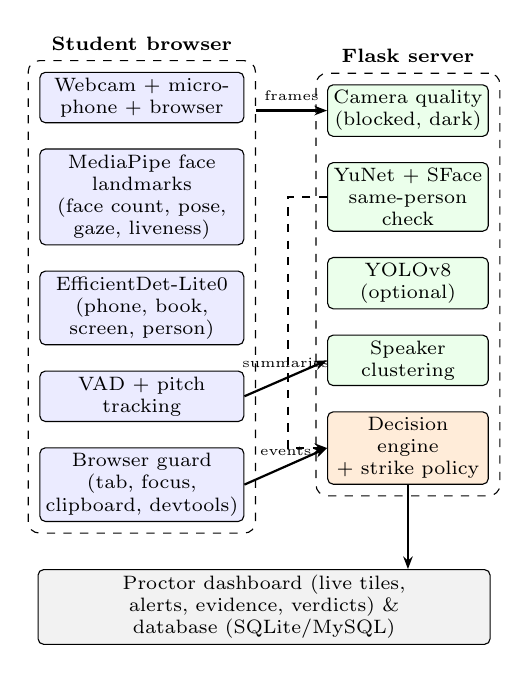
\begin{tikzpicture}[
  node distance=0.32cm and 0.35cm,
  box/.style={draw, rounded corners=2pt, align=center, font=\scriptsize, minimum height=0.55cm, inner sep=2pt, text width=2.45cm},
  sbox/.style={box, text width=1.9cm},
  arr/.style={-{Stealth[length=1.6mm]}, thick}]
\node[box, fill=blue!8] (cam) {Webcam + microphone + browser};
\node[box, fill=blue!8, below=of cam] (mp) {MediaPipe face landmarks\\(face count, pose, gaze, liveness)};
\node[box, fill=blue!8, below=of mp] (od) {EfficientDet-Lite0\\(phone, book, screen, person)};
\node[box, fill=blue!8, below=of od] (au) {VAD + pitch tracking};
\node[box, fill=blue!8, below=of au] (br) {Browser guard\\(tab, focus, clipboard, devtools)};
\begin{scope}[on background layer]
\node[draw, dashed, rounded corners, fit=(cam)(br), inner sep=4pt, label={[font=\scriptsize\bfseries]above:Student browser}] (client) {};
\end{scope}
\node[sbox, fill=green!8, right=1.05cm of mp] (fv) {YuNet + SFace\\same-person check};
\node[sbox, fill=green!8, below=of fv] (yolo) {YOLOv8\\(optional)};
\node[sbox, fill=green!8, below=of yolo] (spk) {Speaker\\clustering};
\node[sbox, fill=orange!15, below=of spk] (eng) {Decision engine\\+ strike policy};
\node[sbox, fill=green!8, above=of fv] (q) {Camera quality\\(blocked, dark)};
\begin{scope}[on background layer]
\node[draw, dashed, rounded corners, fit=(q)(eng), inner sep=4pt, label={[font=\scriptsize\bfseries]above:Flask server}] (srv) {};
\end{scope}
\path (client.south west) -- (srv.south east) coordinate[pos=0.5] (mid);
\node[box, fill=gray!10, text width=5.6cm, anchor=north] (ui) at ([yshift=-0.45cm]mid |- client.south) {Proctor dashboard (live tiles, alerts, evidence, verdicts) \& database (SQLite/MySQL)};
\draw[arr] (client.east |- q) -- node[above, font=\tiny]{frames} (q.west);
\draw[arr] (au.east) -- node[above, font=\tiny]{summaries} (spk.west);
\draw[arr] (br.east) -- node[above, font=\tiny]{events} (eng.west);
\draw[arr] (eng.south) -- (eng.south |- ui.north);
\draw[arr, dashed] (fv.west) -- ++(-0.5,0) |- (eng.west);
\end{tikzpicture}}
\caption{System architecture: on-device analysis gives real-time feedback; the server re-verifies sampled frames, scores the evidence and informs proctors.}
\label{fig:arch}
\end{figure}

\subsection{Roles and Workflow}
\emph{Administrators} manage users, enrol faces, tune the engine weights and inspect analytics and the audit log. \emph{Proctors} create exams (single choice, multiple choice, true/false, short answer and essay, plus CSV import), monitor live tiles sorted by risk, approve identities, warn students, add time, flag or terminate sessions, review events, grade answers and export reports. \emph{Students} register with a webcam photo, complete a pre-exam check, verify their identity and take the exam in full-screen mode. A \emph{written mode} supports paper-based answers: looking down is not penalised and students photograph their answer sheets at the end.

The exam flow is: (1) system check of the camera, microphone, browser features, number of monitors and network latency; (2) rules and consent; (3) a randomized liveness challenge and the start photo; (4) the monitored exam with autosave and a server-authoritative timer; and (5) review, grading and reporting.

\section{Methodology}
\subsection{Identity Enrolment and Start-of-Exam Verification}
At registration, the face is detected and a feature vector $\mathbf{e}_{\text{enr}}$ is stored. The preferred backend is YuNet \cite{wu2023yunet} for detection with SFace \cite{zhong2021sface} for 128-dimensional deep embeddings, compared with cosine similarity:
\begin{equation}
s(\mathbf{a},\mathbf{b}) = \frac{\mathbf{a}^\top\mathbf{b}}{\lVert\mathbf{a}\rVert\,\lVert\mathbf{b}\rVert}.
\end{equation}
When the deep models are not installed, a fallback uses a Haar cascade detector \cite{viola2001rapid} and a $4{\times}4$ spatial histogram of uniform LBP codes \cite{ahonen2006lbp} with Hellinger normalisation; this fallback is less accurate and is labelled as such in the interface. The enrolment photo must contain exactly one sufficiently large face.

Before the start photo is taken, the client issues two random challenges drawn from \{blink twice, turn the head and return, smile, nod\}, which are verified from MediaPipe blendshapes and landmarks to reject printed photos. The start photo $\mathbf{e}_0$ is accepted when $s(\mathbf{e}_{\text{enr}},\mathbf{e}_0)\ge\tau_b$ for the active backend $b$. After three failures the session enters a \emph{pending approval} state in which a proctor compares the registered photo and the start photo side by side; the exam timer starts only after approval. If the active backend changes after enrolment, the stored photo is re-encoded with the new model, so the check is never skipped.

\subsection{Continuous Same-Person Verification}
Every frame uploaded during the exam is compared with the start photo $\mathbf{e}_0$, which was taken in the same room seconds before the exam began. Two mechanisms reduce false alarms:

\emph{Pose gating.} A frame is compared only if it contains exactly one face and both the server landmarks and the browser estimate report $|\psi|\le 20^\circ$ (yaw) and $|\theta|\le 22^\circ$ (pitch). Turned faces are handled by the behaviour detectors instead.

\emph{Per-session baseline.} The mean similarity $\bar{s}$ of the first $N=5$ matching frontal frames is the student's own baseline. A frame is a mismatch when
\begin{equation}
s_t < \min\left(\tau_b,\; \bar{s} - m_b\right),
\end{equation}
where $m_b$ is a backend margin. A \emph{Different person detected} event (critical) is raised after $k_b$ consecutive mismatches ($k=2$ for SFace, $k=3$ for the fallback), with a screenshot attached. With $T_f=5$\,s, a substitution is therefore flagged within $k_bT_f$ seconds, at most 15\,s.

\subsection{Face Presence, Head Pose and Gaze}
The browser runs the MediaPipe Face Landmarker \cite{kartynnik2019facemesh}, which outputs 478 landmarks and 52 blendshapes per face. Yaw is estimated from the horizontal position of the nose tip between the two cheek landmarks, and pitch from the vertical position of the nose between the eye line and the chin. A personal baseline built from the first 80 frontal samples compensates for camera placement. The client reports \emph{head turned} for $|\psi|>22^\circ$ or a pitch outside the allowed band for more than 1.5\,s, \emph{repeated head movement} for five or more turns per minute, and \emph{gaze away} when the eye-direction blendshapes exceed 0.42 horizontally for 2\,s. It also reports \emph{face missing} after 3\,s, \emph{left camera view} after 15\,s and \emph{multiple faces} after 1.5\,s. Because the server's frontal detector can miss a turned face, the server does not report \emph{face missing} when the browser still sees one.

\subsection{Prohibited Objects and Additional Persons}
EfficientDet-Lite0 \cite{tan2020efficientdet} (COCO classes) runs in the browser every 0.7\,s. A phone is reported when one detection has a score of at least 0.6, or when two consecutive frames score at least 0.32. Books are ignored in written mode, and laptops or TVs are reported as an extra device. On the server, YOLOv8n \cite{jocher2023yolov8} checks every uploaded frame when it is installed. A person count greater than one raises \emph{multiple persons}.

\subsection{Audio Analysis}
To preserve privacy, the browser never uploads audio. Every 100\,ms it computes the RMS level against a median noise floor calibrated over the first 3\,s and, for frames above $2.5\times$ the floor, an autocorrelation pitch estimate in the range 70--400\,Hz. Every 5\,s it sends a summary: the voiced ratio, the level in dB above the floor, the loud ratio and the pitch track. The server classifies a window as speech when the voiced ratio is at least 0.25, the level is at least 8\,dB above the floor and there are at least 6 pitch values. It estimates two speakers with 1-D $k$-means ($k{=}2$) when the centroids are separated by at least 35\%, the smaller cluster holds at least 20\% of the values, and the separation exceeds 2.5 times the within-cluster spread.

\subsection{Browser Supervision}
The client records visibility changes (tab switch), window blur (focus lost), full-screen exits (after which a blocking overlay is shown), copy/cut/paste, blocked shortcuts (developer tools, view source, print, save), Print Screen, the window-size gap that indicates docked developer tools, \texttt{screen.isExtended} (multiple monitors), resizing, going offline and camera or microphone tracks ending. The server raises \emph{connection lost} when no heartbeat arrives for 30\,s and accepts only a whitelist of event types from the client; identity and composite events are server-only.

\subsection{Explainable Decision Engine}
Each event $i$ of type $c_i$ has a base weight $w_{c_i}$ (36 event types, editable by the administrator), a confidence $\kappa_i\in[0,1]$ and a timestamp $t_i$. Let $n_i$ be the number of events of the same type up to and including $i$. The raw evidence at time $t$ is
\begin{equation}
R(t)=\sum_{i:\,r_i\neq\text{dismissed}} w_{c_i}\,\rho(n_i)\,\kappa_i\,\delta_{c_i}(t-t_i),
\end{equation}
\begin{equation}
\rho(n)=\min\!\left(2,\,1+0.25(n-1)\right),
\end{equation}
\begin{equation}
\delta_c(\Delta)=\begin{cases}2^{-\Delta/H} & \text{if } c \text{ is behavioural,}\\ 1 & \text{if } c \text{ is hard evidence,}\end{cases}
\end{equation}
with half-life $H=600$\,s. Repetition therefore counts progressively more, minor behaviour fades, and hard evidence (phone, another person, impersonation, blocked camera) never decays. Events confirmed by a proctor use $\kappa_i=1$, and dismissed events are removed. The score is bounded with a saturating map:
\begin{equation}
S(t)=100\left(1-e^{-R(t)/\sigma}\right),\qquad \sigma=50.
\end{equation}
\emph{Correlation rules} add composite events when independent signals co-occur: looking away or face missing within 30\,s of speech gives \emph{suspected assistance}, and leaving the exam window within 20\,s of looking away gives \emph{suspected look-up}. The interface shows the contribution of each category (identity, face, behaviour, object, audio, browser, composite). Each exam sets a warning threshold (default 40) and a critical threshold (default 75), with optional automatic termination.

\subsection{Warnings, Strike Policy and Human Review}
Every medium-or-higher event outside the system, composite and manual categories is a \emph{strike}. The student immediately sees a red banner with an explanation (e.g., ``Mobile phone detected. Put it away immediately.'') and the number of warnings left; reaching the exam's limit (default 10, configurable, 0 for unlimited) ends the exam automatically with the reason shown. Proctors receive the same events live, can send messages, extend time or terminate, and record a final verdict (cleared, suspicious, malpractice) after confirming or dismissing each event. All staff actions are written to an audit log.

\section{Implementation}
The server is written in Python~3 with Flask, Flask-Login, Flask-WTF (CSRF protection) and SQLAlchemy, about 3.7k lines of Python, 1.8k lines of JavaScript and 1.5k lines of Jinja templates. OpenCV~4 provides image decoding, quality checks and the YuNet/SFace and Haar/LBP backends; NumPy implements the audio clustering; Ultralytics YOLOv8 is optional. The client uses the MediaPipe Tasks Vision WebAssembly runtime, which can be self-hosted together with its models by a download script so that exams do not depend on a CDN. Evidence and snapshots are stored on disk and served only to staff or to the student they belong to. Exam times are stored in UTC and displayed in the institution's time zone. Schema additions are applied automatically to existing databases.

\section{Experimental Evaluation}
All measurements were produced by the project's pytest suite, browser end-to-end tests with Playwright and Chromium, and the script \texttt{scripts/evaluate.py}, which writes the figures and \texttt{results.json} used here. Timing was measured on a 4-core Intel Xeon (2.1\,GHz) virtual machine without a GPU, with Python 3.13 and OpenCV 4.14.

\subsection{Automated Test Suite}
Table~\ref{tab:tests} summarises the 32 automated tests, all of which pass. The functional tests drive the real HTTP API with a deterministic stand-in face model, so identity logic (start match, continuous mismatch, pose gating, model change) is tested independently of camera hardware.

\begin{table}[t]
\caption{Automated test suite (32/32 passing)}
\label{tab:tests}
\centering
\footnotesize
\begin{tabular}{@{}p{1.6cm}c p{5.0cm}@{}}
\toprule
\textbf{Group} & \textbf{Tests} & \textbf{What is verified} \\
\midrule
Decision engine \& audio & 9 & zero score for clean sessions; hard evidence outweighs minor events; super-linear repetition; decay of behavioural events only; dismissed events ignored and confirmed ones at full weight; score bounded at 100; administrator weight overrides; correlation rule within its window only; one vs.\ two speakers and silence gating \\
\midrule
End-to-end API flows & 14 & start photo must match the enrolled face; three failures lead to proctor approval; two-person photo rejected; impostor flagged after a sustained mismatch with evidence; blocked camera; turned faces not compared; server trusts the browser when the frontal detector misses; client whitelist and cooldowns; auto-termination at the critical score; strike limit ends the exam; template re-encoded on model change; grading of all objective types; auto-submit at time-out; access control; proctor review recalculates the score; warnings delivered \\
\midrule
Pages \& administration & 9 & every page renders for each role (20+ URLs); CSV export; engine settings round-trip; exam editor with option remapping and CSV import; proctor visibility rules; publishing in local time; student visibility of drafts; seeded scores explainable \\
\bottomrule
\end{tabular}
\end{table}

\subsection{Browser End-to-End Tests}
Chromium was launched with a virtual camera that streams a recorded video, so the real client code (MediaPipe in WebAssembly, frame upload, warning UI) was exercised. Table~\ref{tab:e2e} lists the scenarios and the observed outcomes.

\begin{table}[t]
\caption{Browser end-to-end scenarios (virtual camera)}
\label{tab:e2e}
\centering
\footnotesize
\begin{tabular}{@{}p{3.1cm}p{4.9cm}@{}}
\toprule
\textbf{Scenario} & \textbf{Observed outcome} \\
\midrule
Registration with webcam photo & face enrolled, student dashboard shown \\
Pre-exam system check & camera, browser, display, network and on-device models reported ready \\
Start verification, genuine user & accepted; live similarity 0.98 (fallback backend) \\
Different person replaces student & \emph{Different person detected} (critical) with evidence; student notice and proctor alert; tile and timeline updated \\
Copy attempt (Ctrl+C) & blocked; red warning banner, counter ``1/4'' \\
Strike limit reached (limit 4) & exam ended automatically with the reason shown \\
Proctor/admin dashboards & live tiles, score chart, timeline and reports rendered without errors \\
\bottomrule
\end{tabular}
\end{table}

\subsection{Decision Engine Behaviour}
We replayed six synthetic 45-minute behaviour profiles through the engine, including its correlation rules (Table~\ref{tab:engine}, Fig.~\ref{fig:scores}). The honest profile stays at 0, and occasional glances peak at 10.5 and decay to 4.1. Tab switching briefly crosses the warning level (peak 44.8), but because these events decay the score falls back to 11.4. Talking while looking away triggers two \emph{suspected assistance} composites, which supply 36 of the points. Phone use and impersonation are hard evidence, so their scores stay high until the end of the exam. None of the profiles reaches the critical threshold on its own; this is intended, so that terminating an exam remains a human decision unless an exam enables automatic termination, and the strike policy covers persistent violations.

\begin{table}[t]
\caption{Fraud score for replayed behaviour profiles}
\label{tab:engine}
\centering
\footnotesize
\begin{tabular}{@{}lcccc@{}}
\toprule
\textbf{Profile} & \textbf{Events} & \textbf{Peak} & \textbf{Final} & \textbf{Dominant category} \\
\midrule
Honest student & 0 & 0.0 & 0.0 & -- \\
Occasional glances & 3 & 10.5 & 4.1 & behaviour \\
Tab switching & 5 & 44.8 & 11.4 & browser \\
Talking + looking away & 5+2 & 68.3 & 53.9 & composite \\
Phone usage & 3 & 66.4 & 65.9 & object \\
Impersonation & 3 & 66.9 & 62.6 & identity \\
\bottomrule
\end{tabular}
\end{table}

\begin{figure}[t]
\centering
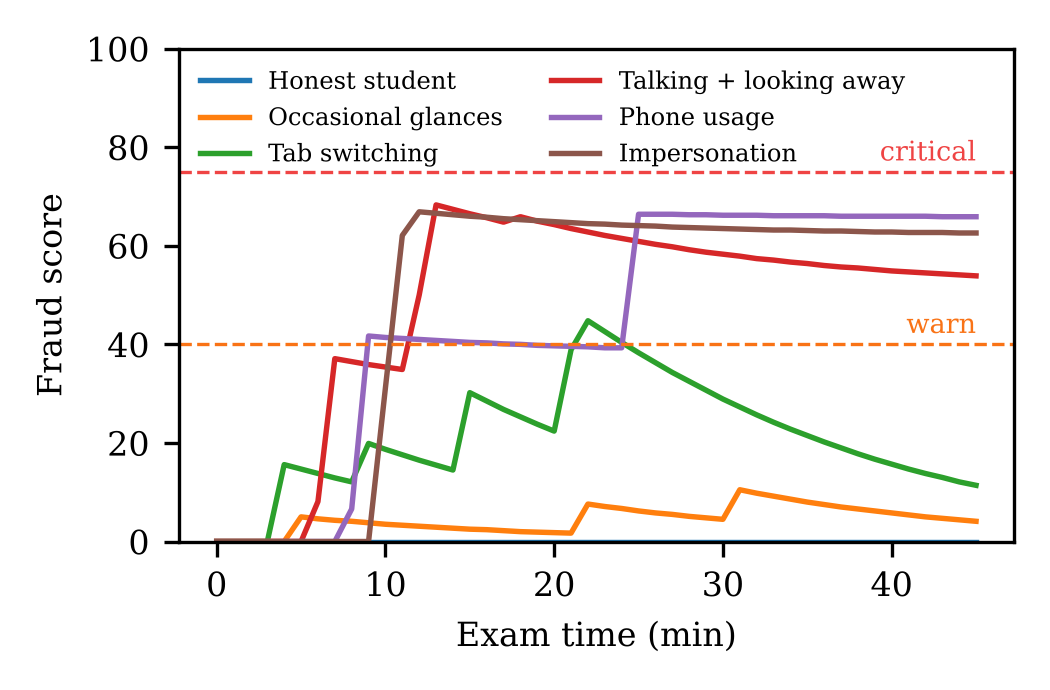
\includegraphics[width=\columnwidth]{fig_scores.png}
\caption{Fraud-score trajectories of the replayed profiles. Behavioural evidence decays; hard evidence persists.}
\label{fig:scores}
\end{figure}

\subsection{Face Verification (Fallback Backend)}
The deep SFace models could not be downloaded in the evaluation environment, so we characterise the fallback matcher, which is what runs before \texttt{download\_models.py} is executed. Two public sample portraits were each augmented 40 times (rotation $\pm8^\circ$, scale 0.75--1.05, translation, brightness/contrast change and noise). This gave 1560 genuine pairs and 1600 impostor pairs (Fig.~\ref{fig:face}). The detection rate was 100\%. Genuine similarity averaged 0.965 (minimum 0.931) and impostor similarity averaged 0.918 (maximum 0.930). At the operating threshold of 0.935, the false accept rate was 0.0\% and the false reject rate 0.5\%. The two distributions are separated by only about 0.05, so with only two identities this is a calibration result, not a biometric benchmark. It motivated the strict threshold, the per-session baseline and the down-weighting of fallback mismatches (reliability 0.6). Evaluating SFace on a public face-verification benchmark is left to future work.

\begin{figure}[t]
\centering
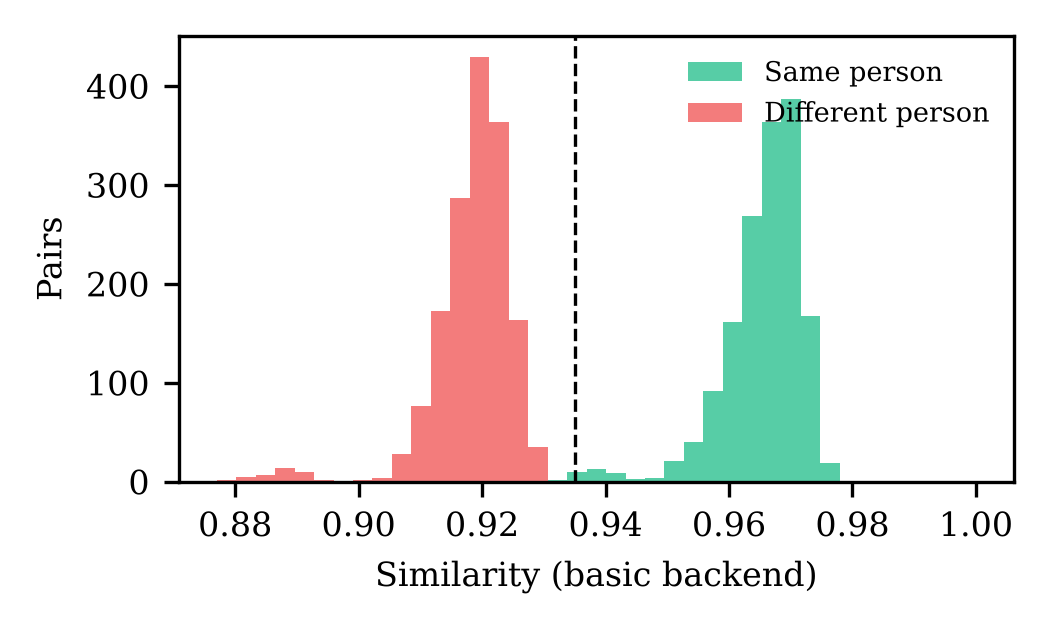
\includegraphics[width=\columnwidth]{fig_face.png}
\caption{Genuine vs.\ impostor similarity of the fallback matcher on augmented sample portraits; dashed line: operating threshold.}
\label{fig:face}
\end{figure}

\subsection{Multiple-Speaker Detection}
We generated 2000 synthetic 5-second pitch tracks: single speakers with a mean F0 between 95 and 240\,Hz and 6\% jitter, and pairs of speakers with any two such voices and a 25--75\% speaking share. Table~\ref{tab:audio} shows that the detector never raised a false alarm on a single speaker (precision 1.00). However, it found only 47.2\% of two-speaker windows (F1 0.64): recall was 100\% when the two pitches differed by more than 35\% (typically a male and a female voice) and 0\% below that. Silence produced no event, and loud non-speech produced only a low-severity \emph{noise} event. The detector is therefore conservative: it rarely accuses a student wrongly, but it misses conversations between people with similar voices. In those cases the system relies on the speech event combined with the correlation rules.

\begin{table}[t]
\caption{Two-speaker detection on 2000 synthetic windows}
\label{tab:audio}
\centering
\footnotesize
\begin{tabular}{@{}lcc@{}}
\toprule
 & \textbf{Predicted 1} & \textbf{Predicted 2} \\
\midrule
True 1 speaker & 1011 & 0 \\
True 2 speakers & 522 & 467 \\
\midrule
\multicolumn{3}{@{}l}{Accuracy 0.739, precision 1.00, recall 0.472, F1 0.641} \\
\bottomrule
\end{tabular}
\end{table}

\subsection{Computational Cost}
Table~\ref{tab:latency} reports the median and 95th-percentile server latency over 60 runs on a 480-pixel-high frame (about 40\,kB as JPEG). A full server analysis takes about 30\,ms and is dominated by face detection. At one frame per 5\,s per student, one CPU core can therefore serve on the order of 150 concurrent candidates with the fallback backend. Scoring 500 events takes under 1\,ms. YOLOv8 adds inference cost on the server when it is enabled.

\begin{table}[t]
\caption{Server processing time per frame (CPU, fallback backend)}
\label{tab:latency}
\centering
\footnotesize
\begin{tabular}{@{}lcc@{}}
\toprule
\textbf{Stage} & \textbf{Median (ms)} & \textbf{P95 (ms)} \\
\midrule
JPEG decode & 0.89 & 0.99 \\
Face detection & 29.7 & 31.2 \\
Face embedding & 0.31 & 0.34 \\
Full frame pipeline (quality, faces, identity) & 30.3 & 32.3 \\
Decision engine, 500 events & 0.75 & 0.79 \\
\bottomrule
\end{tabular}
\end{table}

\section{Discussion and Limitations}
\textbf{What was not measured.} The liveness challenge, real phone detection and speech detection in a real room require physical hardware and were not part of the automated evaluation. The face accuracy reported here is for the fallback backend on two identities. The audio results use synthetic pitch tracks. Validation with real students and an established face benchmark is the most important next step.

\textbf{Evasion.} A browser cannot see other devices on the student's network, and a phone kept entirely outside the camera's view cannot be detected by any webcam-based system. Mitigations include a second camera (the student's phone showing the desk), room scans, answer-timing analytics, per-question time limits and network-level blocking of AI services when exams are taken on campus.

\textbf{Fairness and privacy.} Face models can perform unequally across demographics \cite{coghlan2021ethics}. For this reason the system never makes a final decision on its own: events can be dismissed, the per-session baseline adapts to each student, the fallback backend is down-weighted, and verdicts are recorded by people and audited. Raw audio is never uploaded, and the models are self-hosted.

\section{Conclusion and Future Work}
We presented an open AI proctoring system that keeps verifying, throughout the exam, that the person who started the exam is the person writing it, and that combines deep-learning vision, audio and browser signals into an explainable, human-reviewed fraud score. Tests and benchmarks confirm the intended behaviour and show interactive performance on a CPU, and they also exposed concrete weaknesses that we report openly. Future work includes evaluating SFace on public benchmarks, fine-tuning YOLOv8 on exam-room imagery (phones below the desk, earbuds, smartwatches), a learned speaker-diarisation model for voices of similar pitch, a second-camera mode and typing-behaviour analytics.

\begin{thebibliography}{00}
\bibitem{nigam2021review} A. Nigam, R. Pasricha, T. Singh, and P. Churi, ``A systematic review on AI-based proctoring systems: Past, present and future,'' \emph{Education and Information Technologies}, vol. 26, pp. 6421--6445, 2021.
\bibitem{hussein2020evaluation} M. J. Hussein, J. Yusuf, A. S. Deb, L. Fong, and S. Naidu, ``An evaluation of online proctoring tools,'' \emph{Open Praxis}, vol. 12, no. 4, pp. 509--525, 2020.
\bibitem{coghlan2021ethics} S. Coghlan, T. Miller, and J. Paterson, ``Good proctor or `Big Brother'? Ethics of online exam supervision technologies,'' \emph{Philosophy \& Technology}, vol. 34, pp. 1581--1606, 2021.
\bibitem{atoum2017automated} Y. Atoum, L. Chen, A. X. Liu, S. D. H. Hsu, and X. Liu, ``Automated online exam proctoring,'' \emph{IEEE Transactions on Multimedia}, vol. 19, no. 7, pp. 1609--1624, 2017.
\bibitem{viola2001rapid} P. Viola and M. Jones, ``Rapid object detection using a boosted cascade of simple features,'' in \emph{Proc. IEEE CVPR}, 2001, pp. I-511--I-518.
\bibitem{ahonen2006lbp} T. Ahonen, A. Hadid, and M. Pietik\"ainen, ``Face description with local binary patterns: Application to face recognition,'' \emph{IEEE Trans. Pattern Analysis and Machine Intelligence}, vol. 28, no. 12, pp. 2037--2041, 2006.
\bibitem{wu2023yunet} W. Wu, H. Peng, and S. Yu, ``YuNet: A tiny millisecond-level face detector,'' \emph{Machine Intelligence Research}, vol. 20, pp. 656--665, 2023.
\bibitem{zhong2021sface} Y. Zhong, W. Deng, J. Hu, D. Zhao, X. Li, and D. Wen, ``SFace: Sigmoid-constrained hypersphere loss for robust face recognition,'' \emph{IEEE Transactions on Image Processing}, vol. 30, pp. 2587--2598, 2021.
\bibitem{lugaresi2019mediapipe} C. Lugaresi \emph{et al.}, ``MediaPipe: A framework for building perception pipelines,'' arXiv:1906.08172, 2019.
\bibitem{kartynnik2019facemesh} Y. Kartynnik, A. Ablavatski, I. Grishchenko, and M. Grundmann, ``Real-time facial surface geometry from monocular video on mobile GPUs,'' arXiv:1907.06724, 2019.
\bibitem{redmon2016yolo} J. Redmon, S. Divvala, R. Girshick, and A. Farhadi, ``You only look once: Unified, real-time object detection,'' in \emph{Proc. IEEE CVPR}, 2016, pp. 779--788.
\bibitem{jocher2023yolov8} G. Jocher, A. Chaurasia, and J. Qiu, ``Ultralytics YOLOv8,'' software, version 8.0, 2023. [Online]. Available: \url{https://github.com/ultralytics/ultralytics}
\bibitem{tan2020efficientdet} M. Tan, R. Pang, and Q. V. Le, ``EfficientDet: Scalable and efficient object detection,'' in \emph{Proc. IEEE/CVF CVPR}, 2020, pp. 10781--10790.
\end{thebibliography}

\end{document}
